\section{Bedeutung für SHA-256}

Die Versuche aus Kapitel \ref{chp:bewertung} und Abschnitt \ref{sec:vergleich} zeigen, dass sich innerhalb eines Tages
ein Urbild für einen \glos{hash} berechnen lässt, der je nach Implementierung mit 18 bis 20 festgelegten Bits beginnt. Das ist jedoch
kein Vergleich zum Ergebnis, das sich durch reines Probieren erzielen lässt. In der Testumgebung können 720.000 \glospl{hash} pro Sekunde
berechnet werden. Damit ist es möglich innerhalb eines Tages ein Urbild für einen \glos{hash} mit bis zu 35 festgelegten Bits zu finden.

\subsection{Initialwertberechnung}
Abschnitt \ref{sec:initialwertberechnung} beschreibt den Sinn einer Initialwertberechnung. Diese wird im folgenden separat
betrachtet, da die Erweiterung der Eingabe (siehe Abschnitt \ref{sec:sha256:erweiterung}) vollständig berechnet werden kann
und somit durch einen SAT-Solver nicht mehr betrachtet werden braucht. Das Problem reduziert sich damit auf die Berechnung
der 64 Runden. Abbildung \ref{fig:eval_initial} zeigt das Ergebnis dieses Versuchs im Vergleich zur Urbildberechnung.
\begin{figure}[!h]
  \centering
  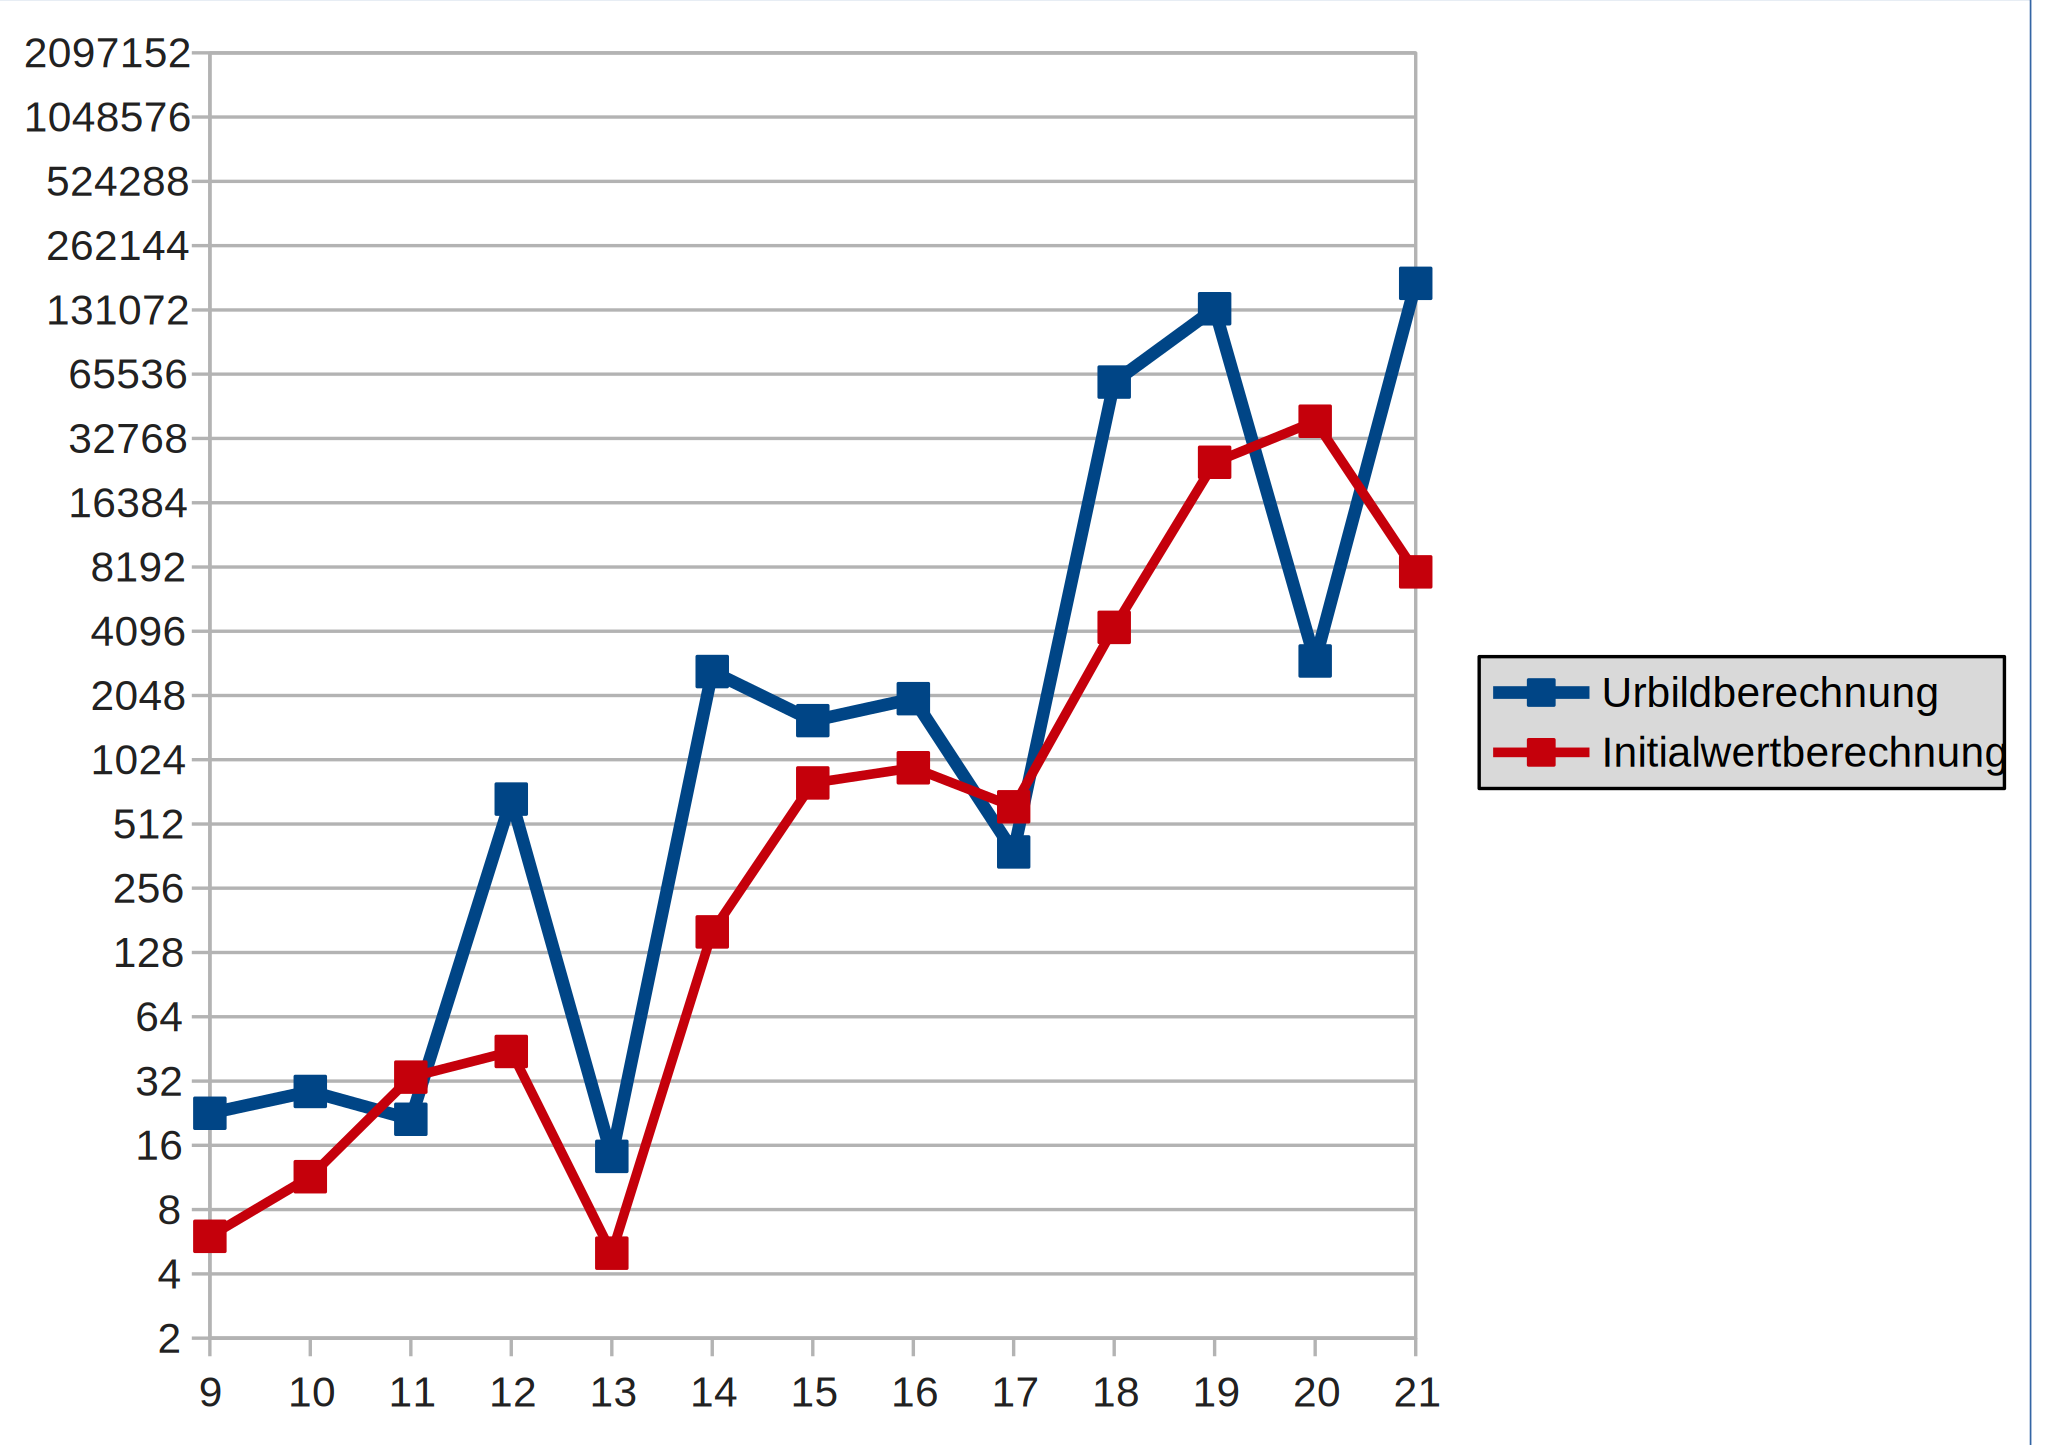
\includegraphics[scale=0.55]{images/eval_initial}
  \caption{Evaluation - Initialwertberechnung}
  \label{fig:eval_initial}
\end{figure}

Während die Urbildbrechnung insgesamt 105 Stunden benötigt hat, wurde die Initialwertberechnung in 22 Stunden
abgeschlossen. Mit drei Ausnahmen war die Initialwertberechnung in allen Fällen schneller als die Urbildberechnung.

\subsection{Kollisionsberechnung}
Abschließend wird die in Abschnitt \ref{sec:kollisionsberechnung} beschriebene Kollisionsberechnung durchgeführt.
Abbildung \ref{fig:eval_kollision} zeigt das Ergebnis im Vergleich zur Urbildberechnung. \clearpage
\begin{figure}[!h]
  \centering
  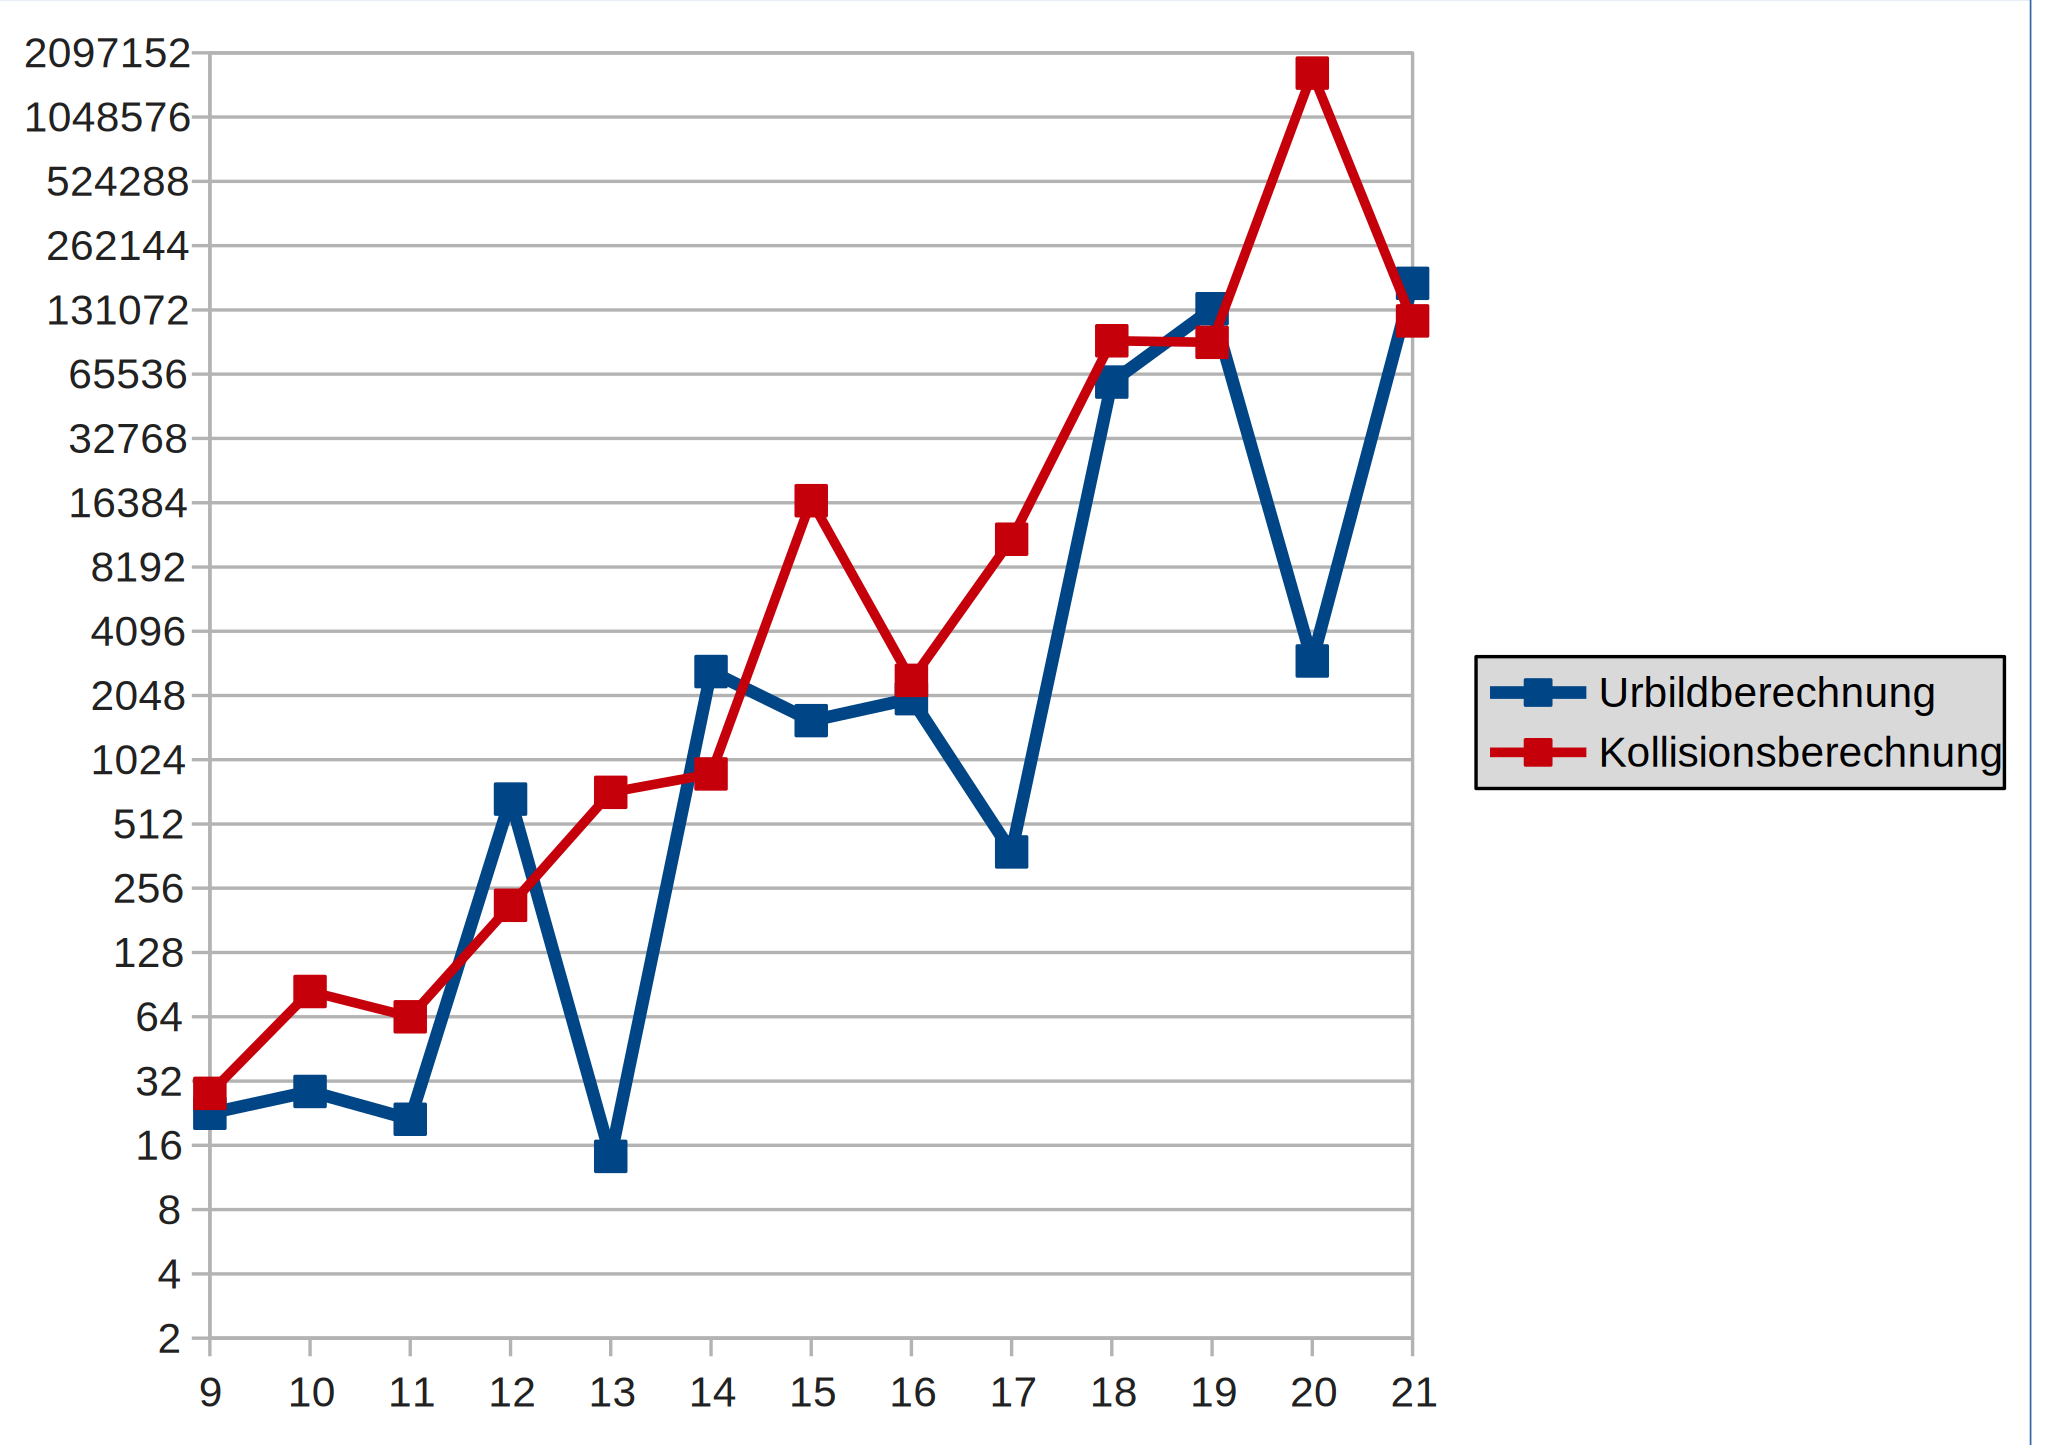
\includegraphics[scale=0.55]{images/eval_kollision}
  \caption{Evaluation - Kollisionsberechnung}
  \label{fig:eval_kollision}
\end{figure}

Es zeigt sich, dass die freie Wahl eines \glos{hash} für CryptoMiniSat keinen Vorteil darstellt. In den meisten Fällen
dauert eine Kollisionsberechnung länger als eine Urbildberechnung. \TODO{Grafik aktualisieren}